\documentclass[11pt]{article}
\usepackage[textwidth=18.0cm, textheight=23.0cm, top=2.0cm]{geometry}
\usepackage{pst-all}
\usepackage{amssymb}
\usepackage{tikz}
\usepackage{underscore}\begin{document}
\pagestyle{empty}


ClassName: \underline{\textbf{Class_03.2bp-30}}
\par
BinSize: \underline{\textbf{40 × 40}}
\par
ReduceSize: \underline{\textbf{40 × 40}}
\par
TypeNum: \underline{\textbf{79}}
\par
Num: \underline{\textbf{80}}
\par
OutS: \underline{\textbf{27200}}
\par
InS: \underline{\textbf{24257}}
\par
Rate: \underline{\textbf{0.892}}
\par
UB: \underline{\textbf{17}}
\par
LB0: \underline{\textbf{17}}
\par
LB: \underline{\textbf{17}}
\par
LBWithCut: \underline{\textbf{17}}
\par
NodeCut: \underline{\textbf{0}}
\par
ExtendedNodeCnt: \underline{\textbf{1}}
\par
GenNodeCnt: \underline{\textbf{1}}
\par
PrimalNode: \underline{\textbf{0}}
\par
ColumnCount: \underline{\textbf{17}}
\par
TotalCutCount: \underline{\textbf{0}}
\par
RootCutCount: \underline{\textbf{0}}
\par
LPSolverCnt: \underline{\textbf{1}}
\par
PricingSolverCnt: \underline{\textbf{0}}
\par
BranchAndBoundNum: \underline{\textbf{1}}
\par
isOpt: \underline{\textbf{true}}
\par
TimeOnInitSolution: \underline{\textbf{600.000 s}}
\par
TimeOnPrimal: \underline{\textbf{0.000 s}}
\par
TimeOnPricing: \underline{\textbf{0.000 s}}
\par
TimeOnRmp: \underline{\textbf{0.078 s}}
\par
TotalTime: \underline{\textbf{600.344 s}}
\par
\newpage


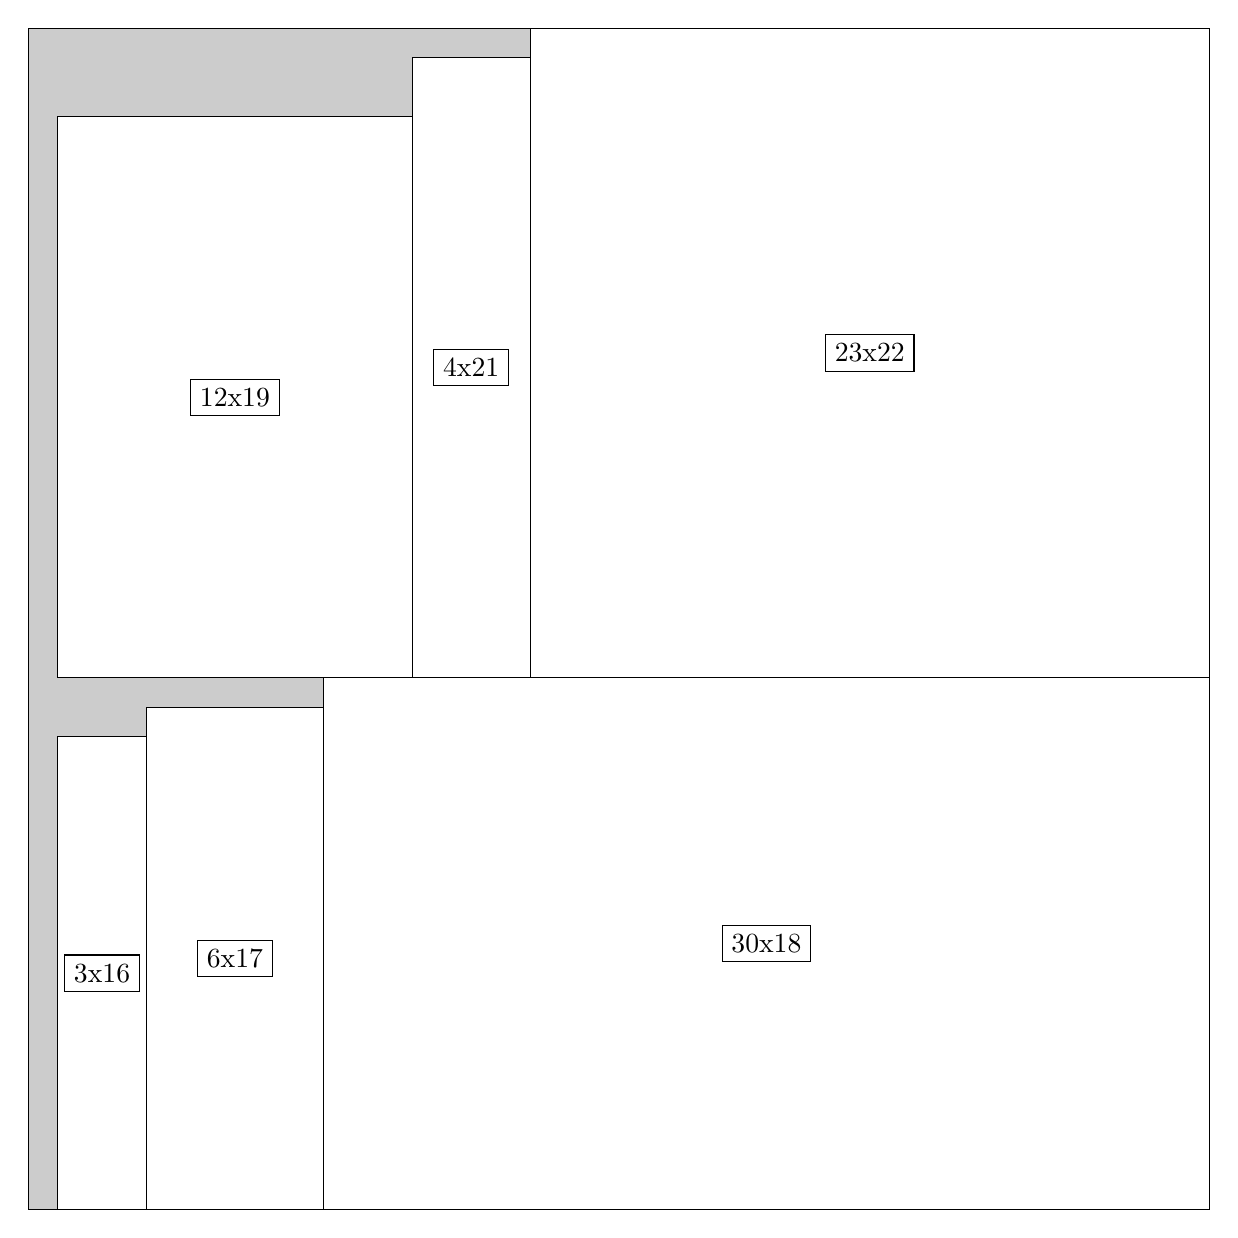
\begin{tikzpicture}[shorten >=1pt,scale=1.0,every node/.style={scale=1.0},->]
\tikzstyle{vertex}=[circle,fill=black!25,minimum size=14pt,inner sep=0pt]
\filldraw[fill=gray!40!white, draw=black] (0,0) rectangle (15.0,15.0);
\foreach \name/\x/\y/\w/\h in {30x18/3.75/0.0/11.25/6.75,6x17/1.5/0.0/2.25/6.375,3x16/0.375/0.0/1.125/6.0,23x22/6.375/6.75/8.625/8.25,4x21/4.875/6.75/1.5/7.875,12x19/0.375/6.75/4.5/7.125}
\filldraw[fill=white!40!white, draw=black] (\x,\y) rectangle node[draw] (\name) {\name} ++(\w,\h);
\end{tikzpicture}


w =30 , h =18 , x =10 , y =0 , v =540
\par
w =6 , h =17 , x =4 , y =0 , v =102
\par
w =3 , h =16 , x =1 , y =0 , v =48
\par
w =23 , h =22 , x =17 , y =18 , v =506
\par
w =4 , h =21 , x =13 , y =18 , v =84
\par
w =12 , h =19 , x =1 , y =18 , v =228
\par
\newpage


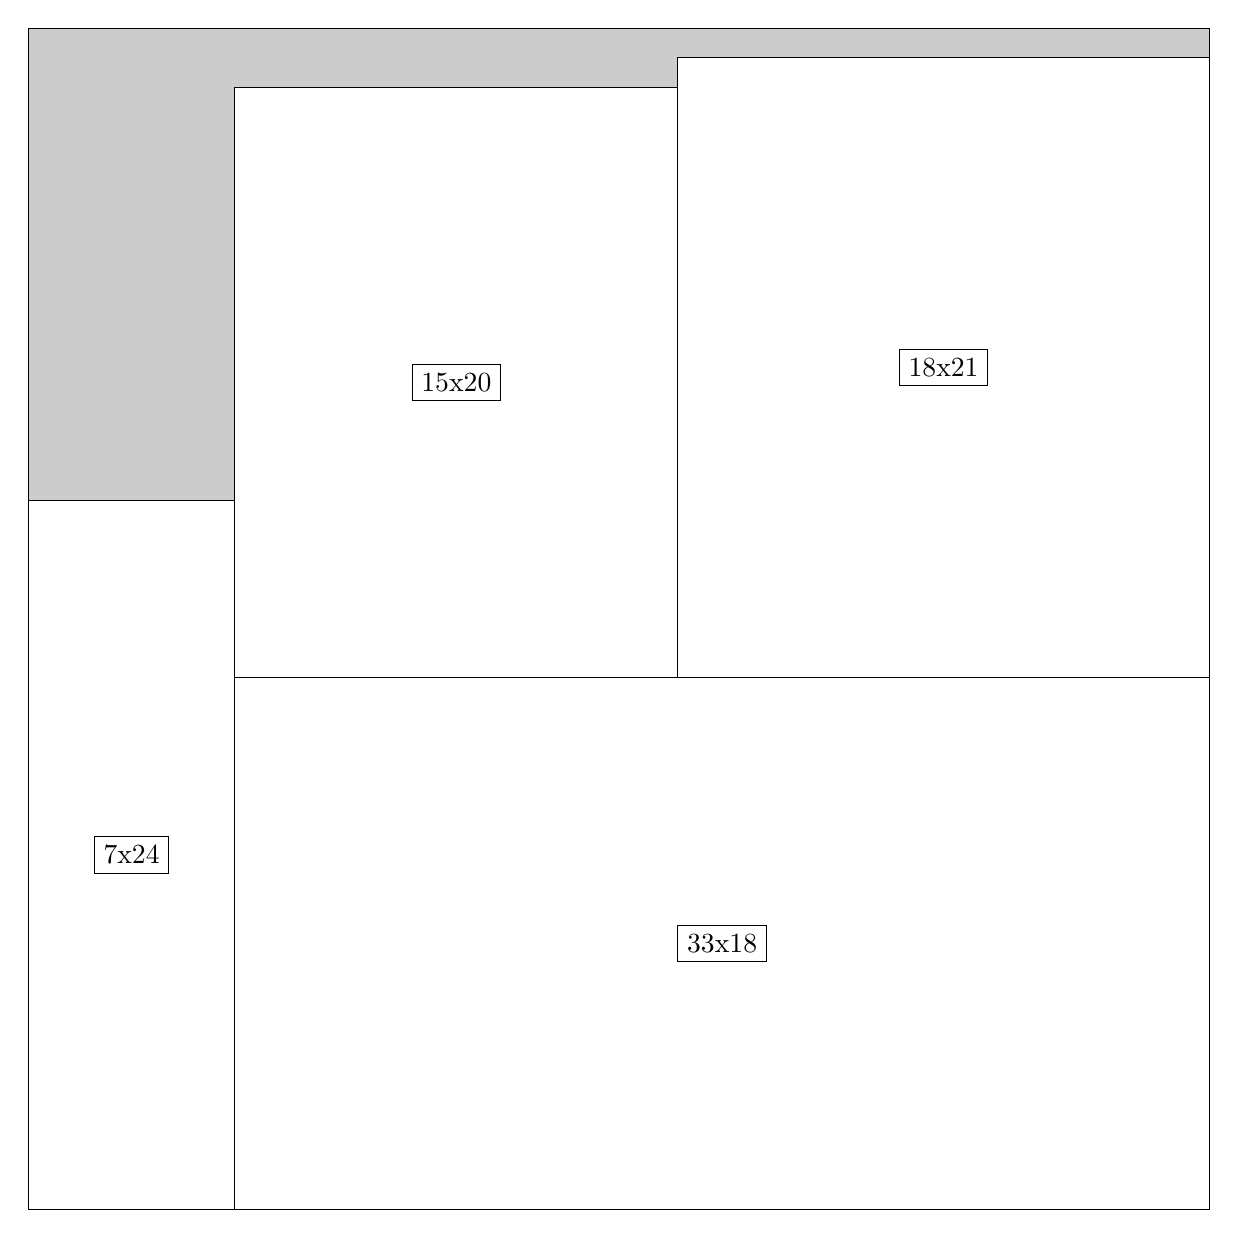
\begin{tikzpicture}[shorten >=1pt,scale=1.0,every node/.style={scale=1.0},->]
\tikzstyle{vertex}=[circle,fill=black!25,minimum size=14pt,inner sep=0pt]
\filldraw[fill=gray!40!white, draw=black] (0,0) rectangle (15.0,15.0);
\foreach \name/\x/\y/\w/\h in {33x18/2.625/0.0/12.375/6.75,18x21/8.25/6.75/6.75/7.875,15x20/2.625/6.75/5.625/7.5,7x24/0.0/0.0/2.625/9.0}
\filldraw[fill=white!40!white, draw=black] (\x,\y) rectangle node[draw] (\name) {\name} ++(\w,\h);
\end{tikzpicture}


w =33 , h =18 , x =7 , y =0 , v =594
\par
w =18 , h =21 , x =22 , y =18 , v =378
\par
w =15 , h =20 , x =7 , y =18 , v =300
\par
w =7 , h =24 , x =0 , y =0 , v =168
\par
\newpage


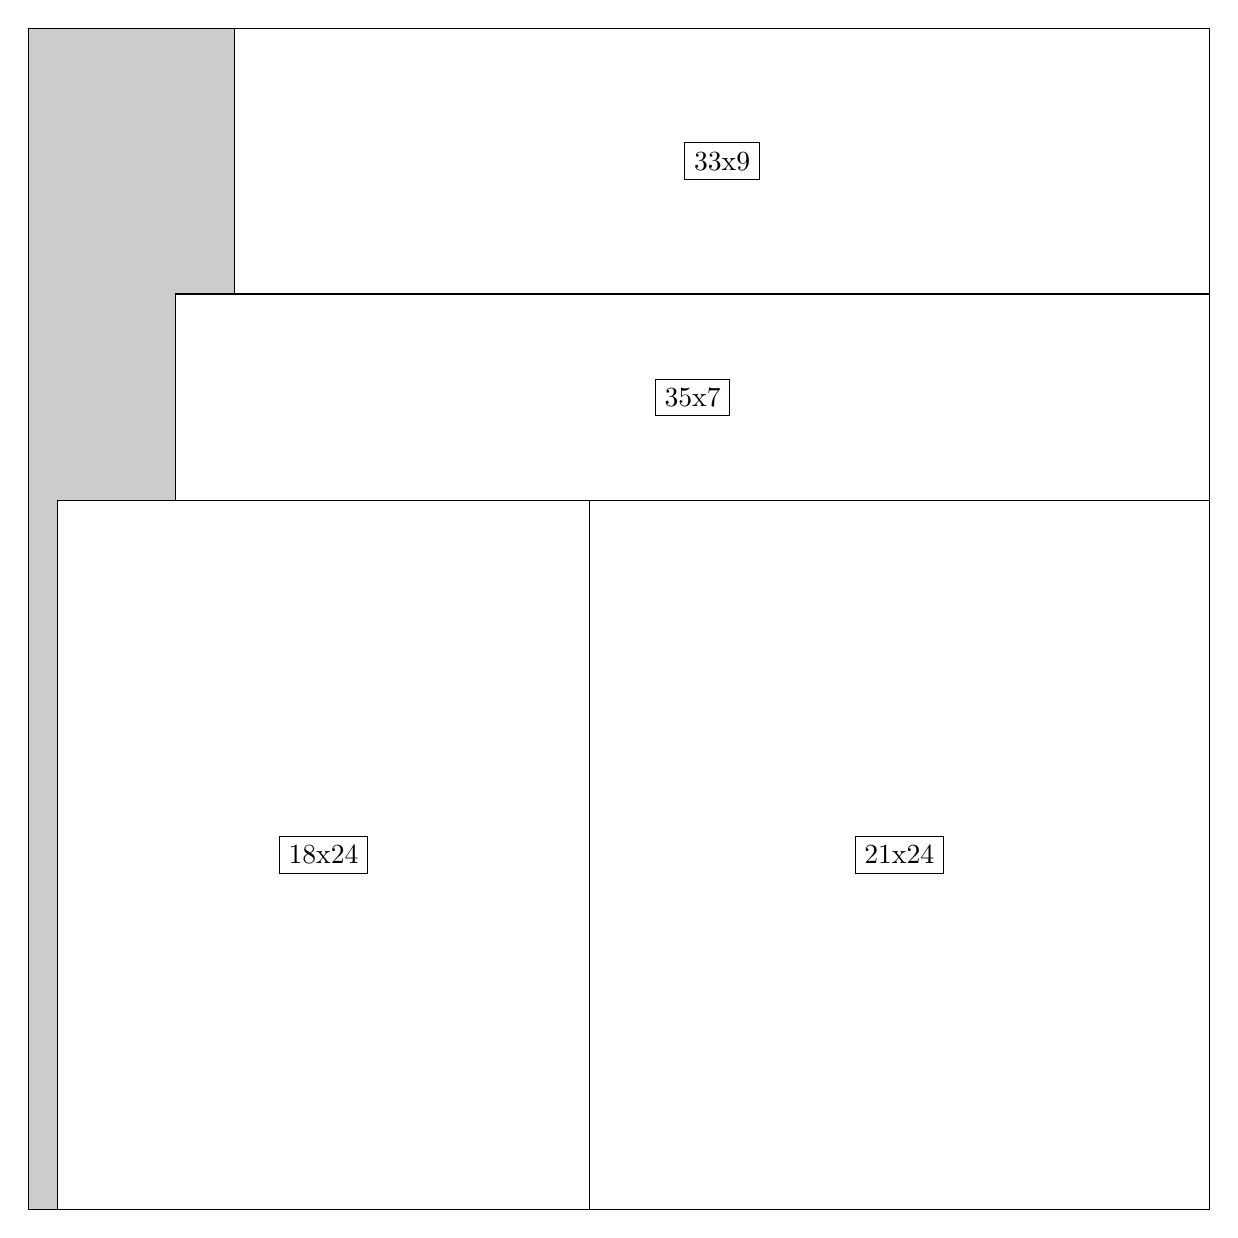
\begin{tikzpicture}[shorten >=1pt,scale=1.0,every node/.style={scale=1.0},->]
\tikzstyle{vertex}=[circle,fill=black!25,minimum size=14pt,inner sep=0pt]
\filldraw[fill=gray!40!white, draw=black] (0,0) rectangle (15.0,15.0);
\foreach \name/\x/\y/\w/\h in {21x24/7.125/0.0/7.875/9.0,18x24/0.375/0.0/6.75/9.0,35x7/1.875/9.0/13.125/2.625,33x9/2.625/11.625/12.375/3.375}
\filldraw[fill=white!40!white, draw=black] (\x,\y) rectangle node[draw] (\name) {\name} ++(\w,\h);
\end{tikzpicture}


w =21 , h =24 , x =19 , y =0 , v =504
\par
w =18 , h =24 , x =1 , y =0 , v =432
\par
w =35 , h =7 , x =5 , y =24 , v =245
\par
w =33 , h =9 , x =7 , y =31 , v =297
\par
\newpage


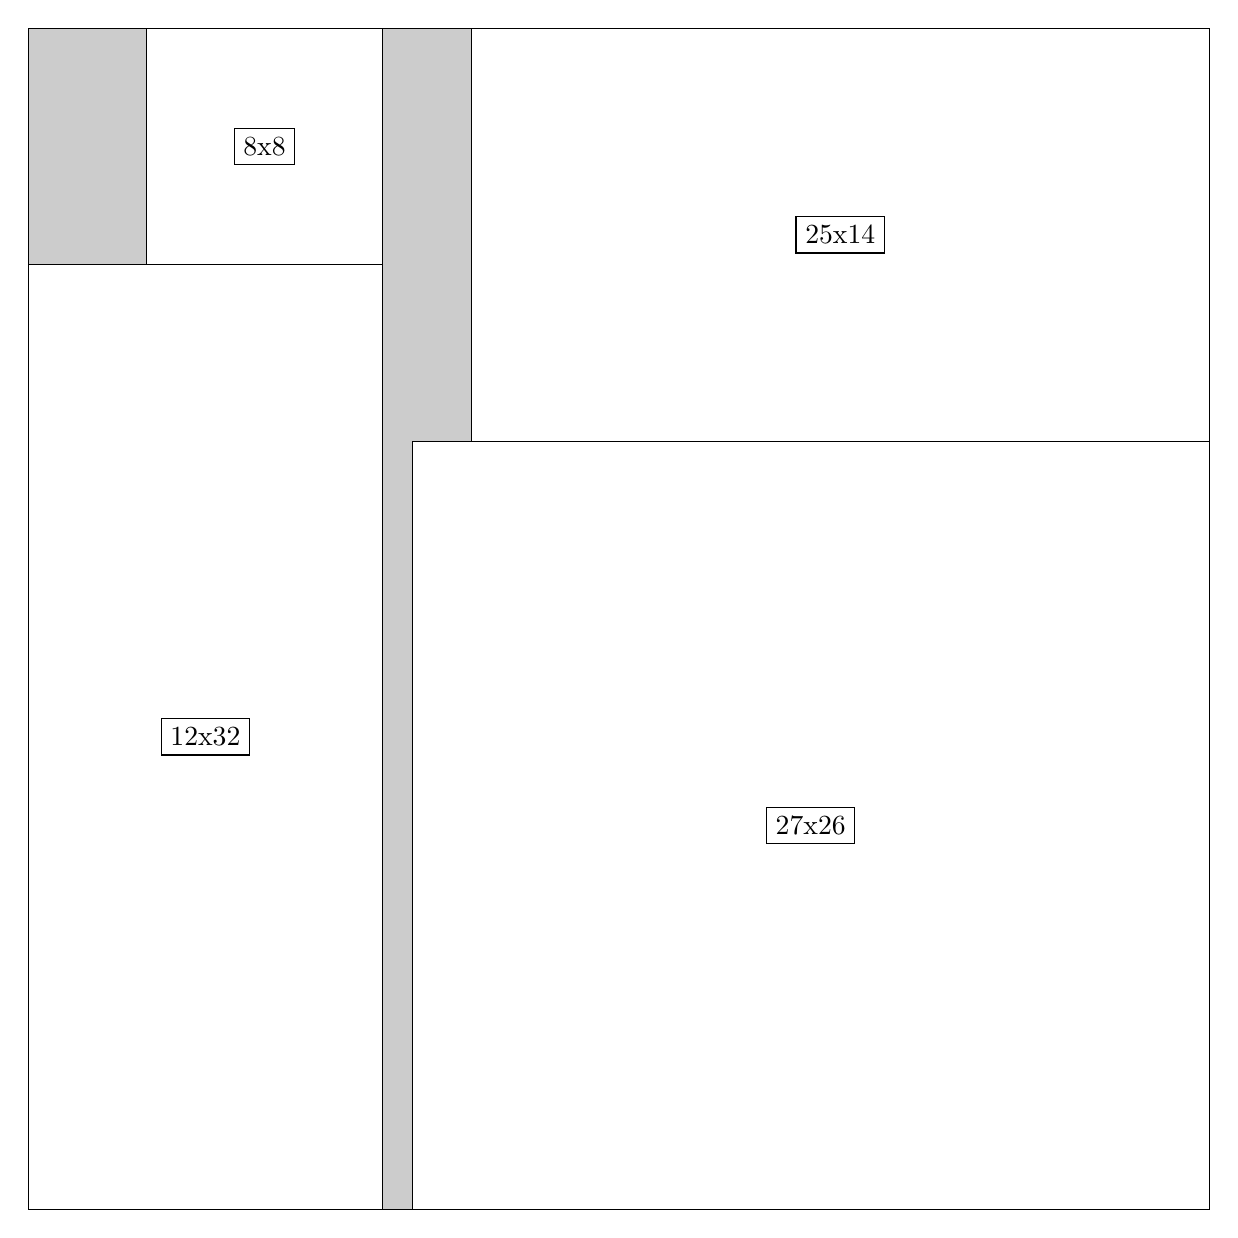
\begin{tikzpicture}[shorten >=1pt,scale=1.0,every node/.style={scale=1.0},->]
\tikzstyle{vertex}=[circle,fill=black!25,minimum size=14pt,inner sep=0pt]
\filldraw[fill=gray!40!white, draw=black] (0,0) rectangle (15.0,15.0);
\foreach \name/\x/\y/\w/\h in {27x26/4.875/0.0/10.125/9.75,25x14/5.625/9.75/9.375/5.25,12x32/0.0/0.0/4.5/12.0,8x8/1.5/12.0/3.0/3.0}
\filldraw[fill=white!40!white, draw=black] (\x,\y) rectangle node[draw] (\name) {\name} ++(\w,\h);
\end{tikzpicture}


w =27 , h =26 , x =13 , y =0 , v =702
\par
w =25 , h =14 , x =15 , y =26 , v =350
\par
w =12 , h =32 , x =0 , y =0 , v =384
\par
w =8 , h =8 , x =4 , y =32 , v =64
\par
\newpage


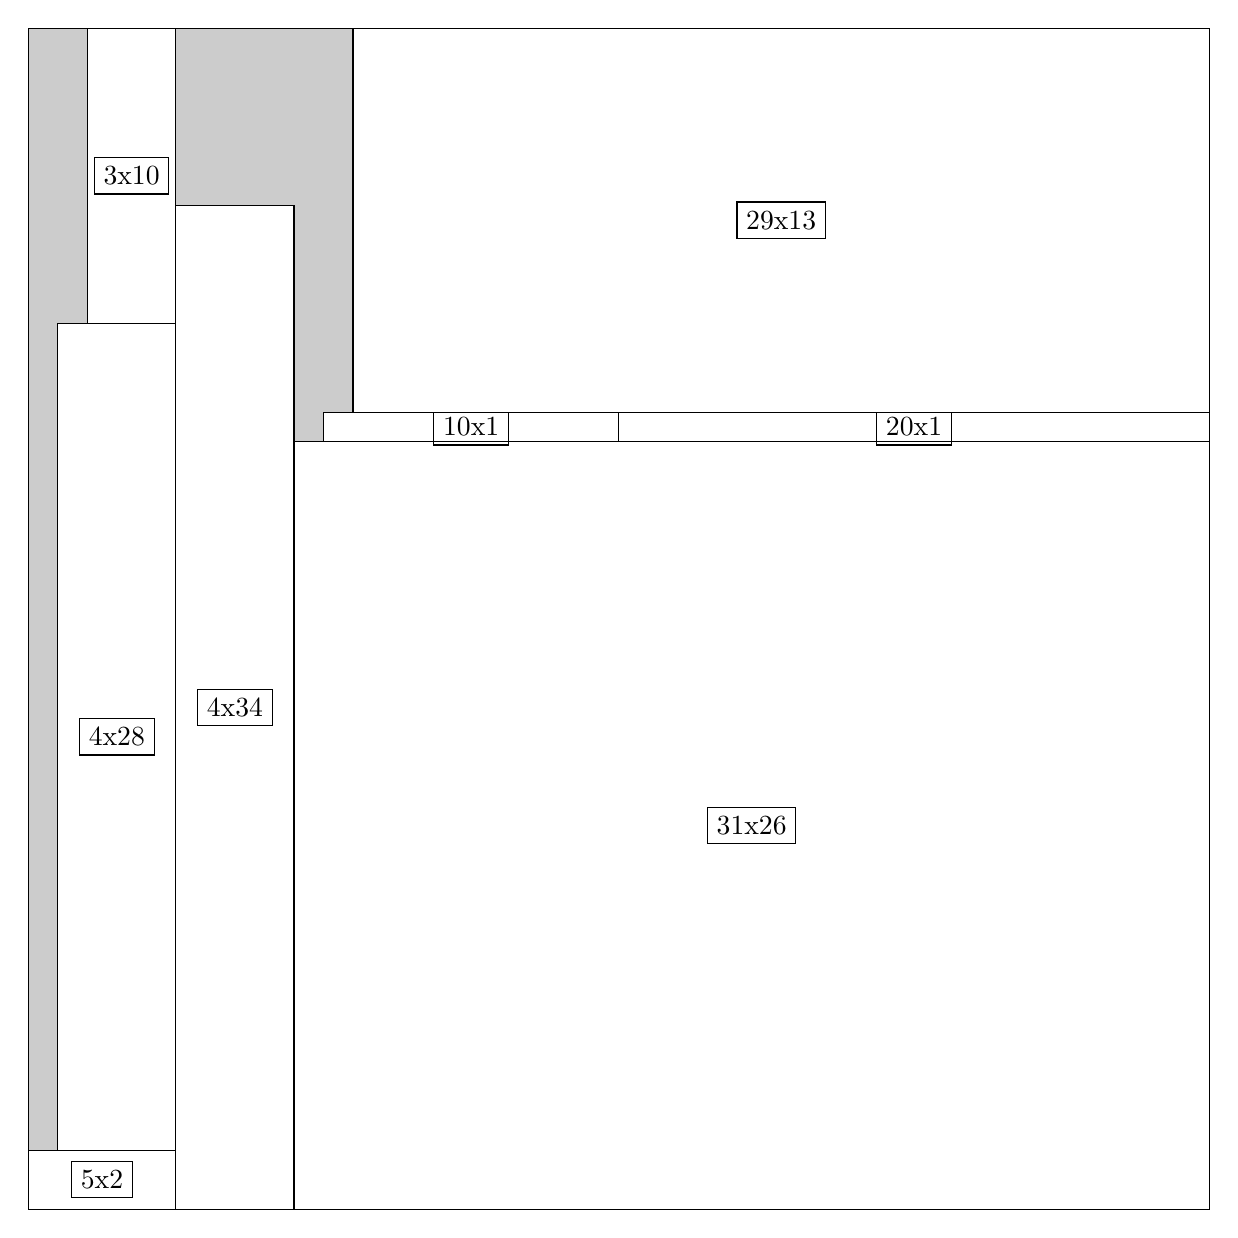
\begin{tikzpicture}[shorten >=1pt,scale=1.0,every node/.style={scale=1.0},->]
\tikzstyle{vertex}=[circle,fill=black!25,minimum size=14pt,inner sep=0pt]
\filldraw[fill=gray!40!white, draw=black] (0,0) rectangle (15.0,15.0);
\foreach \name/\x/\y/\w/\h in {31x26/3.375/0.0/11.625/9.75,20x1/7.5/9.75/7.5/0.375,10x1/3.75/9.75/3.75/0.375,29x13/4.125/10.125/10.875/4.875,4x34/1.875/0.0/1.5/12.75,5x2/0.0/0.0/1.875/0.75,4x28/0.375/0.75/1.5/10.5,3x10/0.75/11.25/1.125/3.75}
\filldraw[fill=white!40!white, draw=black] (\x,\y) rectangle node[draw] (\name) {\name} ++(\w,\h);
\end{tikzpicture}


w =31 , h =26 , x =9 , y =0 , v =806
\par
w =20 , h =1 , x =20 , y =26 , v =20
\par
w =10 , h =1 , x =10 , y =26 , v =10
\par
w =29 , h =13 , x =11 , y =27 , v =377
\par
w =4 , h =34 , x =5 , y =0 , v =136
\par
w =5 , h =2 , x =0 , y =0 , v =10
\par
w =4 , h =28 , x =1 , y =2 , v =112
\par
w =3 , h =10 , x =2 , y =30 , v =30
\par
\newpage


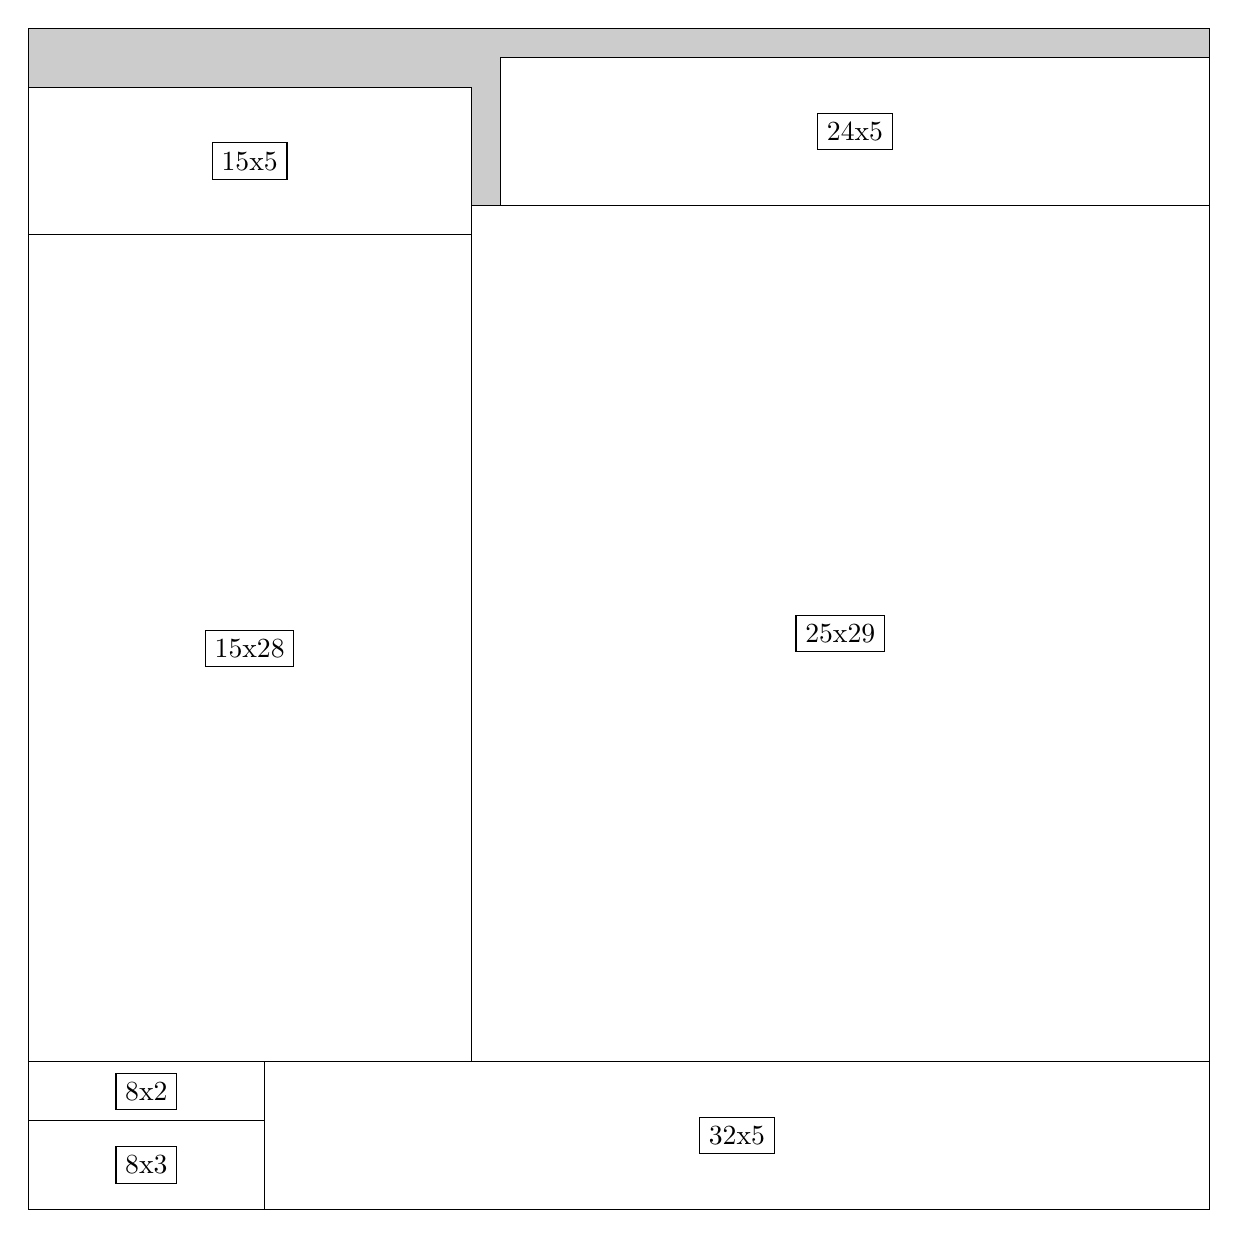
\begin{tikzpicture}[shorten >=1pt,scale=1.0,every node/.style={scale=1.0},->]
\tikzstyle{vertex}=[circle,fill=black!25,minimum size=14pt,inner sep=0pt]
\filldraw[fill=gray!40!white, draw=black] (0,0) rectangle (15.0,15.0);
\foreach \name/\x/\y/\w/\h in {32x5/3.0/0.0/12.0/1.875,8x3/0.0/0.0/3.0/1.125,8x2/0.0/1.125/3.0/0.75,25x29/5.625/1.875/9.375/10.875,24x5/6.0/12.75/9.0/1.875,15x28/0.0/1.875/5.625/10.5,15x5/0.0/12.375/5.625/1.875}
\filldraw[fill=white!40!white, draw=black] (\x,\y) rectangle node[draw] (\name) {\name} ++(\w,\h);
\end{tikzpicture}


w =32 , h =5 , x =8 , y =0 , v =160
\par
w =8 , h =3 , x =0 , y =0 , v =24
\par
w =8 , h =2 , x =0 , y =3 , v =16
\par
w =25 , h =29 , x =15 , y =5 , v =725
\par
w =24 , h =5 , x =16 , y =34 , v =120
\par
w =15 , h =28 , x =0 , y =5 , v =420
\par
w =15 , h =5 , x =0 , y =33 , v =75
\par
\newpage


\begin{tikzpicture}[shorten >=1pt,scale=1.0,every node/.style={scale=1.0},->]
\tikzstyle{vertex}=[circle,fill=black!25,minimum size=14pt,inner sep=0pt]
\filldraw[fill=gray!40!white, draw=black] (0,0) rectangle (15.0,15.0);
\foreach \name/\x/\y/\w/\h in {20x22/7.5/0.0/7.5/8.25,20x18/7.5/8.25/7.5/6.75,20x29/0.0/0.0/7.5/10.875,19x11/0.375/10.875/7.125/4.125}
\filldraw[fill=white!40!white, draw=black] (\x,\y) rectangle node[draw] (\name) {\name} ++(\w,\h);
\end{tikzpicture}


w =20 , h =22 , x =20 , y =0 , v =440
\par
w =20 , h =18 , x =20 , y =22 , v =360
\par
w =20 , h =29 , x =0 , y =0 , v =580
\par
w =19 , h =11 , x =1 , y =29 , v =209
\par
\newpage


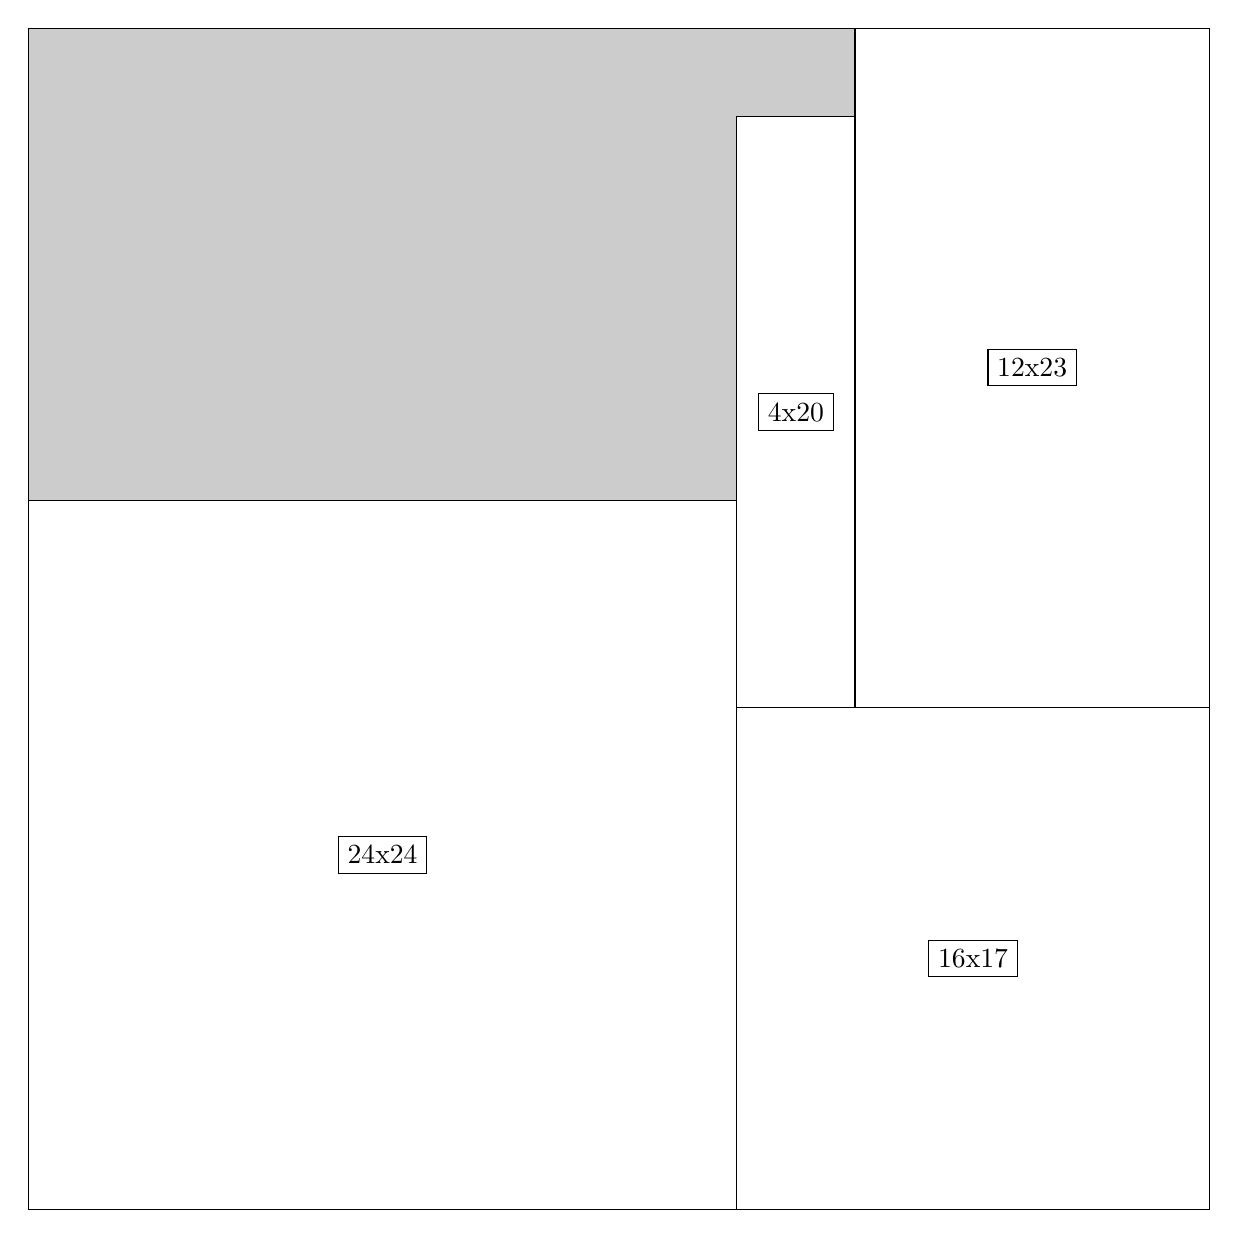
\begin{tikzpicture}[shorten >=1pt,scale=1.0,every node/.style={scale=1.0},->]
\tikzstyle{vertex}=[circle,fill=black!25,minimum size=14pt,inner sep=0pt]
\filldraw[fill=gray!40!white, draw=black] (0,0) rectangle (15.0,15.0);
\foreach \name/\x/\y/\w/\h in {16x17/9.0/0.0/6.0/6.375,12x23/10.5/6.375/4.5/8.625,4x20/9.0/6.375/1.5/7.5,24x24/0.0/0.0/9.0/9.0}
\filldraw[fill=white!40!white, draw=black] (\x,\y) rectangle node[draw] (\name) {\name} ++(\w,\h);
\end{tikzpicture}


w =16 , h =17 , x =24 , y =0 , v =272
\par
w =12 , h =23 , x =28 , y =17 , v =276
\par
w =4 , h =20 , x =24 , y =17 , v =80
\par
w =24 , h =24 , x =0 , y =0 , v =576
\par
\newpage


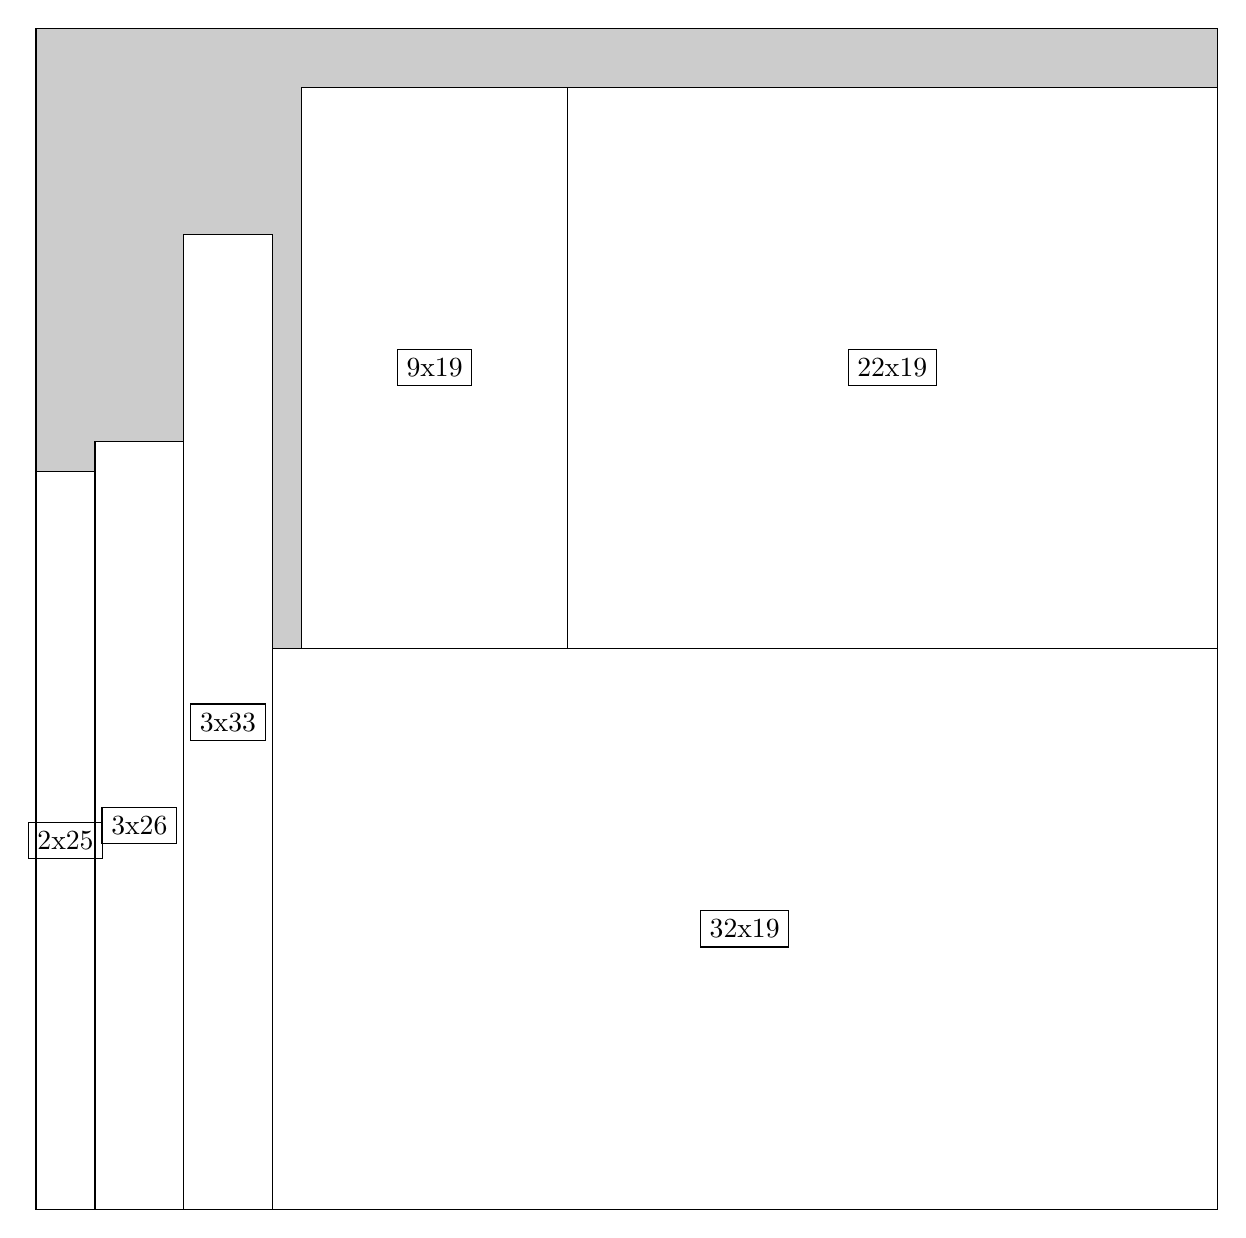
\begin{tikzpicture}[shorten >=1pt,scale=1.0,every node/.style={scale=1.0},->]
\tikzstyle{vertex}=[circle,fill=black!25,minimum size=14pt,inner sep=0pt]
\filldraw[fill=gray!40!white, draw=black] (0,0) rectangle (15.0,15.0);
\foreach \name/\x/\y/\w/\h in {32x19/3.0/0.0/12.0/7.125,22x19/6.75/7.125/8.25/7.125,9x19/3.375/7.125/3.375/7.125,3x33/1.875/0.0/1.125/12.375,3x26/0.75/0.0/1.125/9.75,2x25/0.0/0.0/0.75/9.375}
\filldraw[fill=white!40!white, draw=black] (\x,\y) rectangle node[draw] (\name) {\name} ++(\w,\h);
\end{tikzpicture}


w =32 , h =19 , x =8 , y =0 , v =608
\par
w =22 , h =19 , x =18 , y =19 , v =418
\par
w =9 , h =19 , x =9 , y =19 , v =171
\par
w =3 , h =33 , x =5 , y =0 , v =99
\par
w =3 , h =26 , x =2 , y =0 , v =78
\par
w =2 , h =25 , x =0 , y =0 , v =50
\par
\newpage


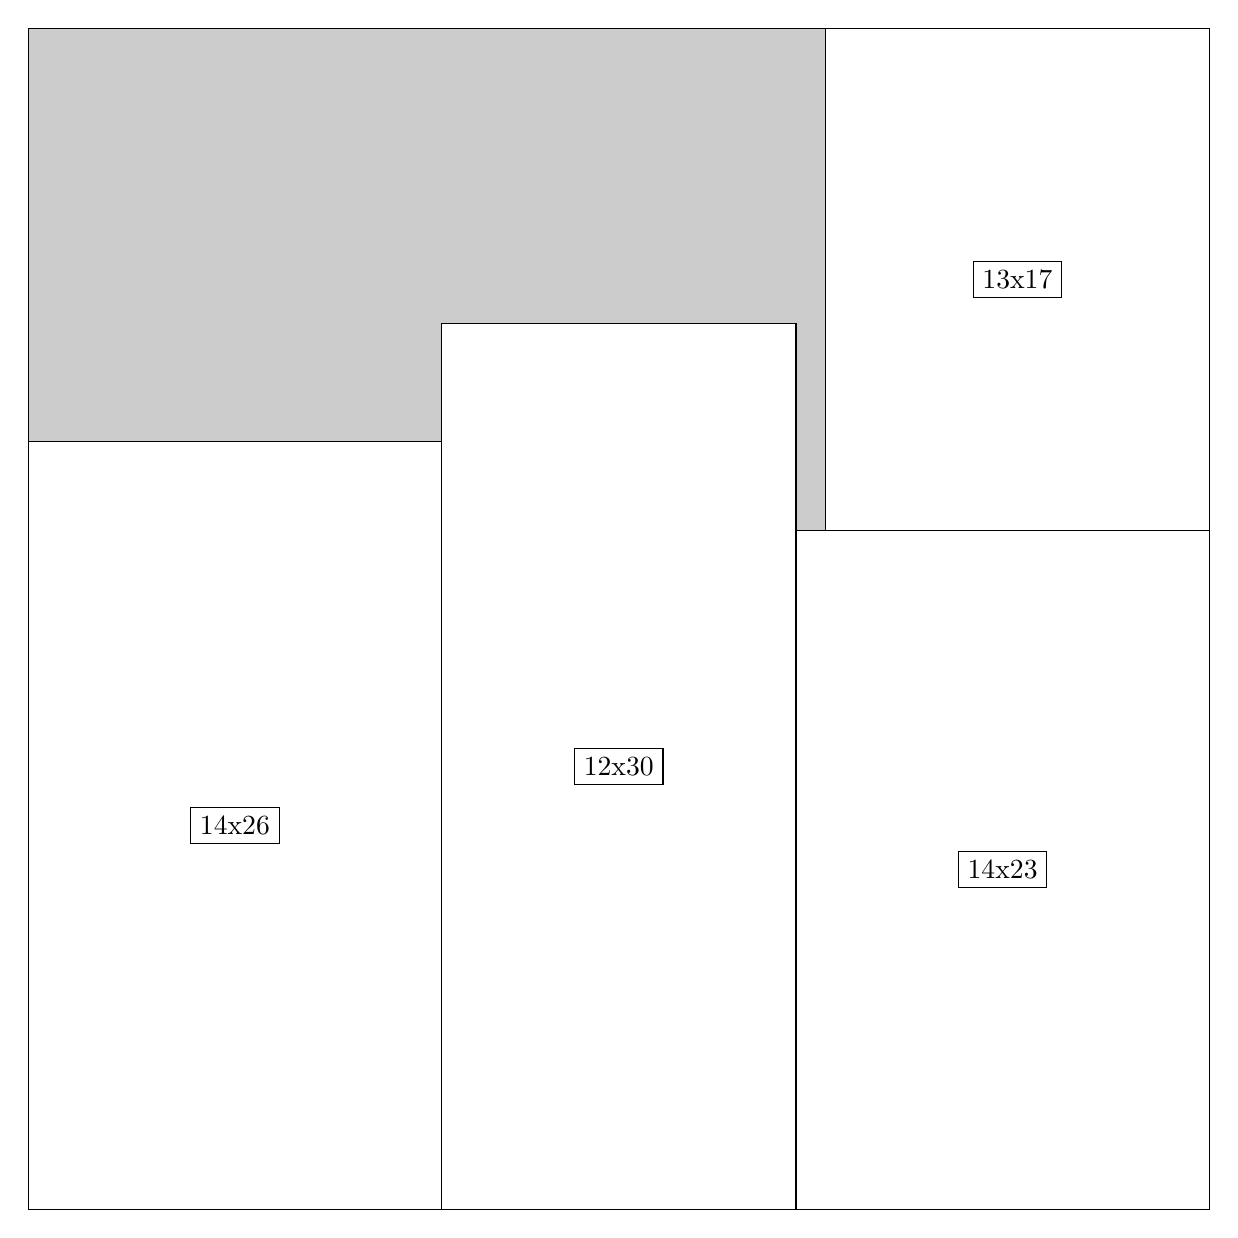
\begin{tikzpicture}[shorten >=1pt,scale=1.0,every node/.style={scale=1.0},->]
\tikzstyle{vertex}=[circle,fill=black!25,minimum size=14pt,inner sep=0pt]
\filldraw[fill=gray!40!white, draw=black] (0,0) rectangle (15.0,15.0);
\foreach \name/\x/\y/\w/\h in {14x23/9.75/0.0/5.25/8.625,13x17/10.125/8.625/4.875/6.375,12x30/5.25/0.0/4.5/11.25,14x26/0.0/0.0/5.25/9.75}
\filldraw[fill=white!40!white, draw=black] (\x,\y) rectangle node[draw] (\name) {\name} ++(\w,\h);
\end{tikzpicture}


w =14 , h =23 , x =26 , y =0 , v =322
\par
w =13 , h =17 , x =27 , y =23 , v =221
\par
w =12 , h =30 , x =14 , y =0 , v =360
\par
w =14 , h =26 , x =0 , y =0 , v =364
\par
\newpage


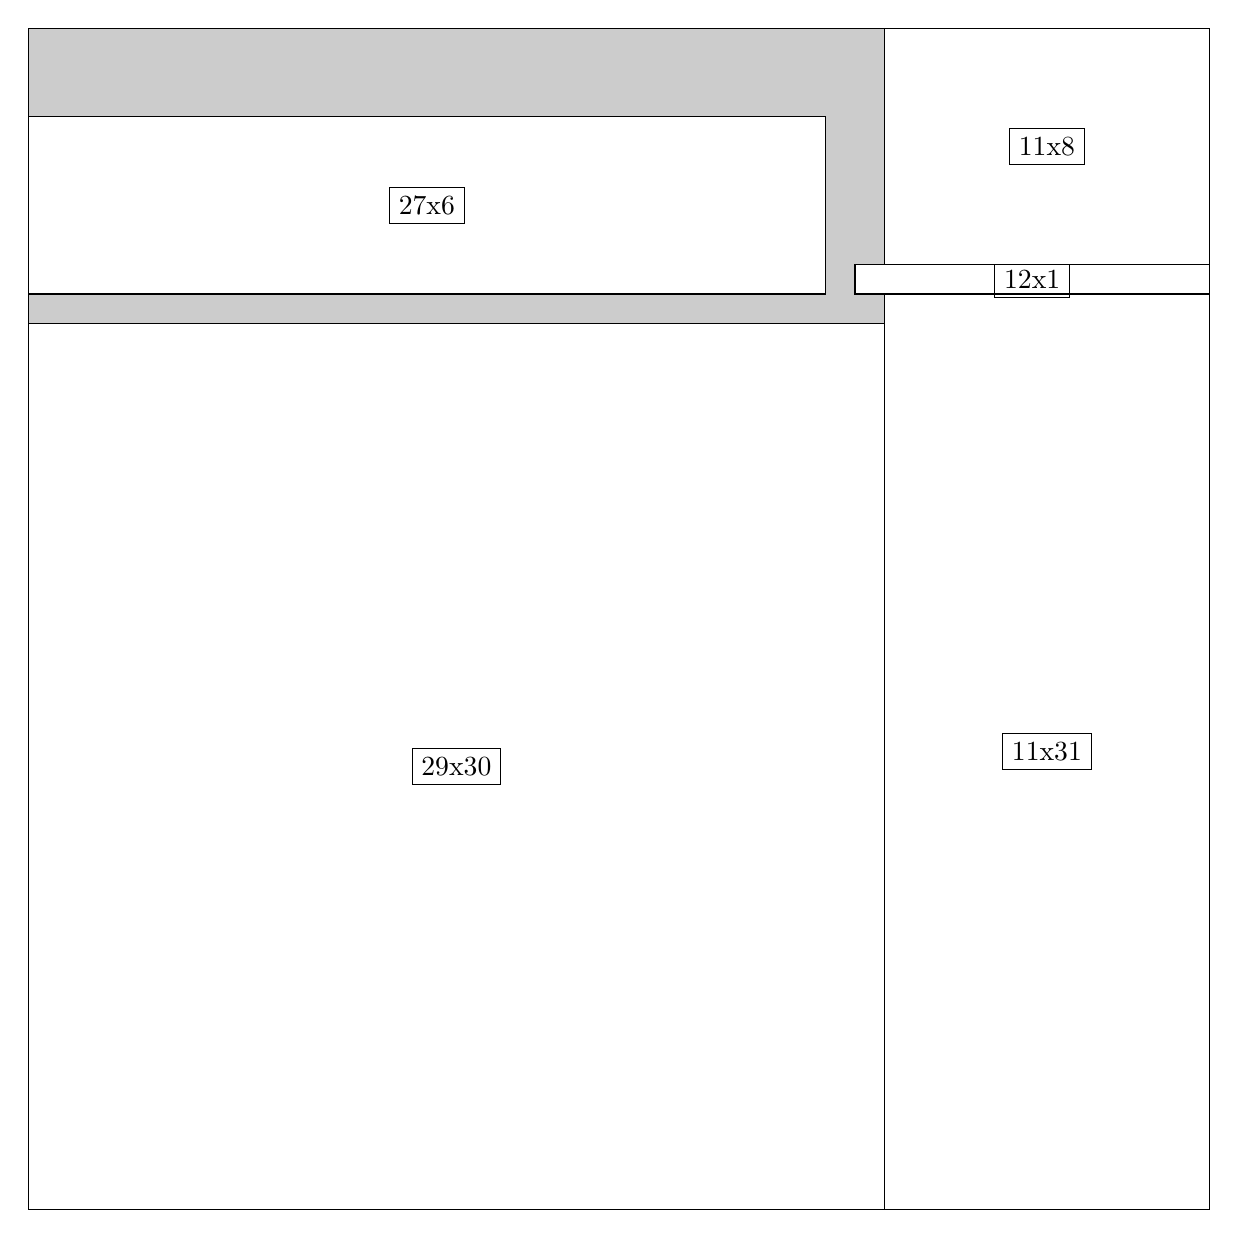
\begin{tikzpicture}[shorten >=1pt,scale=1.0,every node/.style={scale=1.0},->]
\tikzstyle{vertex}=[circle,fill=black!25,minimum size=14pt,inner sep=0pt]
\filldraw[fill=gray!40!white, draw=black] (0,0) rectangle (15.0,15.0);
\foreach \name/\x/\y/\w/\h in {11x31/10.875/0.0/4.125/11.625,29x30/0.0/0.0/10.875/11.25,12x1/10.5/11.625/4.5/0.375,11x8/10.875/12.0/4.125/3.0,27x6/0.0/11.625/10.125/2.25}
\filldraw[fill=white!40!white, draw=black] (\x,\y) rectangle node[draw] (\name) {\name} ++(\w,\h);
\end{tikzpicture}


w =11 , h =31 , x =29 , y =0 , v =341
\par
w =29 , h =30 , x =0 , y =0 , v =870
\par
w =12 , h =1 , x =28 , y =31 , v =12
\par
w =11 , h =8 , x =29 , y =32 , v =88
\par
w =27 , h =6 , x =0 , y =31 , v =162
\par
\newpage


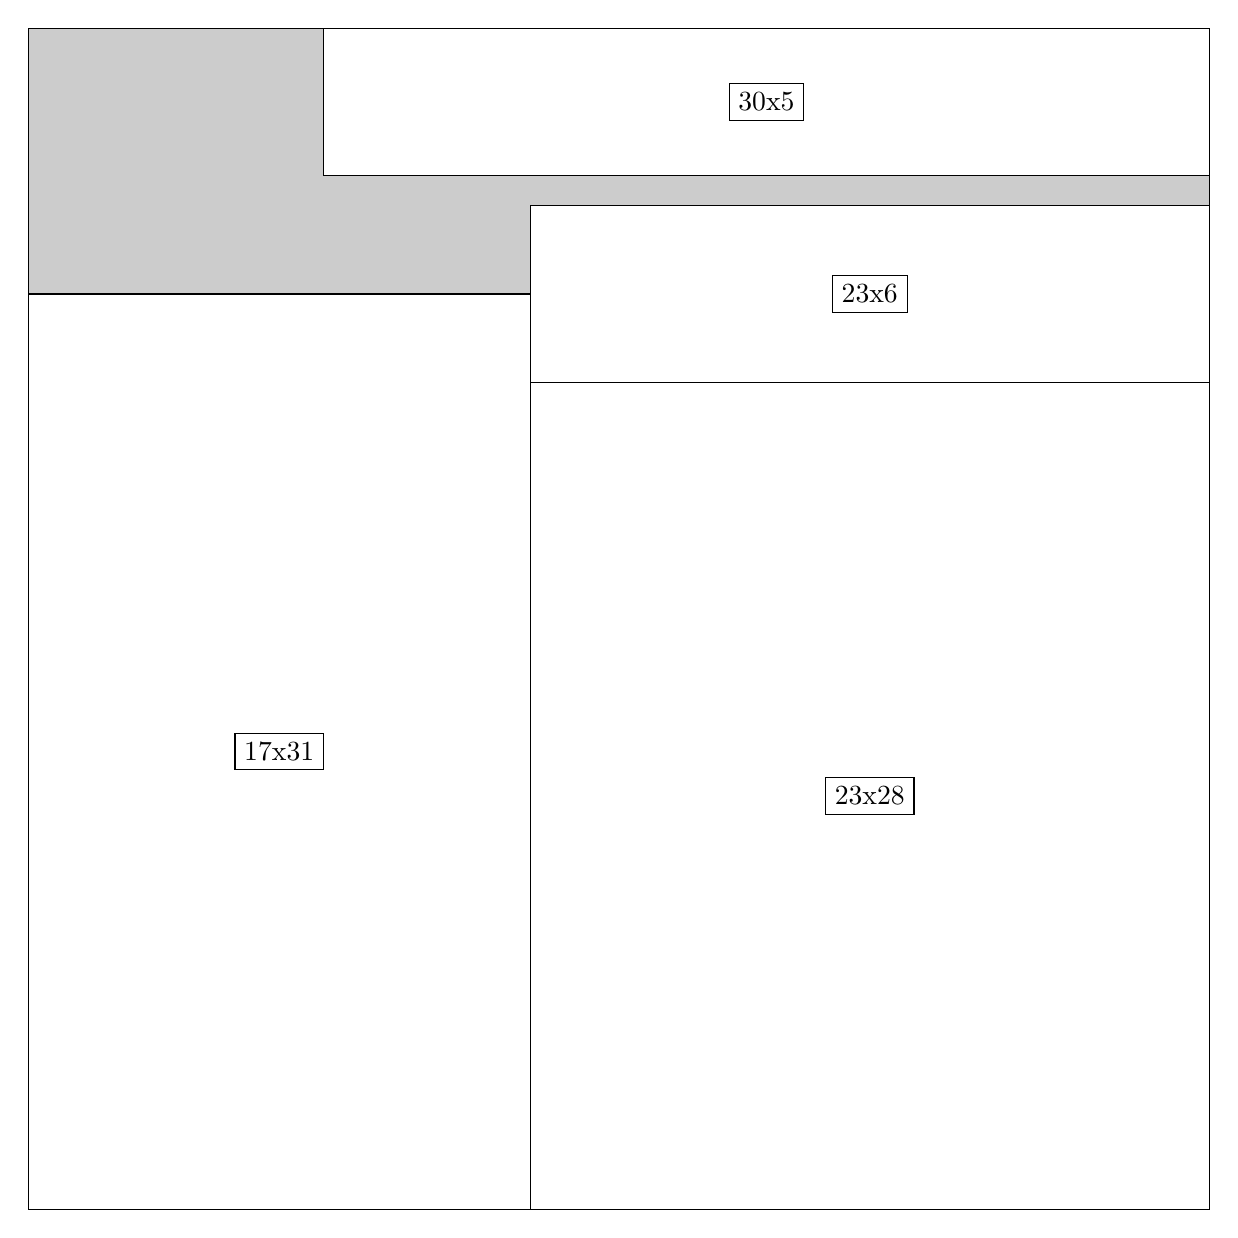
\begin{tikzpicture}[shorten >=1pt,scale=1.0,every node/.style={scale=1.0},->]
\tikzstyle{vertex}=[circle,fill=black!25,minimum size=14pt,inner sep=0pt]
\filldraw[fill=gray!40!white, draw=black] (0,0) rectangle (15.0,15.0);
\foreach \name/\x/\y/\w/\h in {23x28/6.375/0.0/8.625/10.5,23x6/6.375/10.5/8.625/2.25,17x31/0.0/0.0/6.375/11.625,30x5/3.75/13.125/11.25/1.875}
\filldraw[fill=white!40!white, draw=black] (\x,\y) rectangle node[draw] (\name) {\name} ++(\w,\h);
\end{tikzpicture}


w =23 , h =28 , x =17 , y =0 , v =644
\par
w =23 , h =6 , x =17 , y =28 , v =138
\par
w =17 , h =31 , x =0 , y =0 , v =527
\par
w =30 , h =5 , x =10 , y =35 , v =150
\par
\newpage


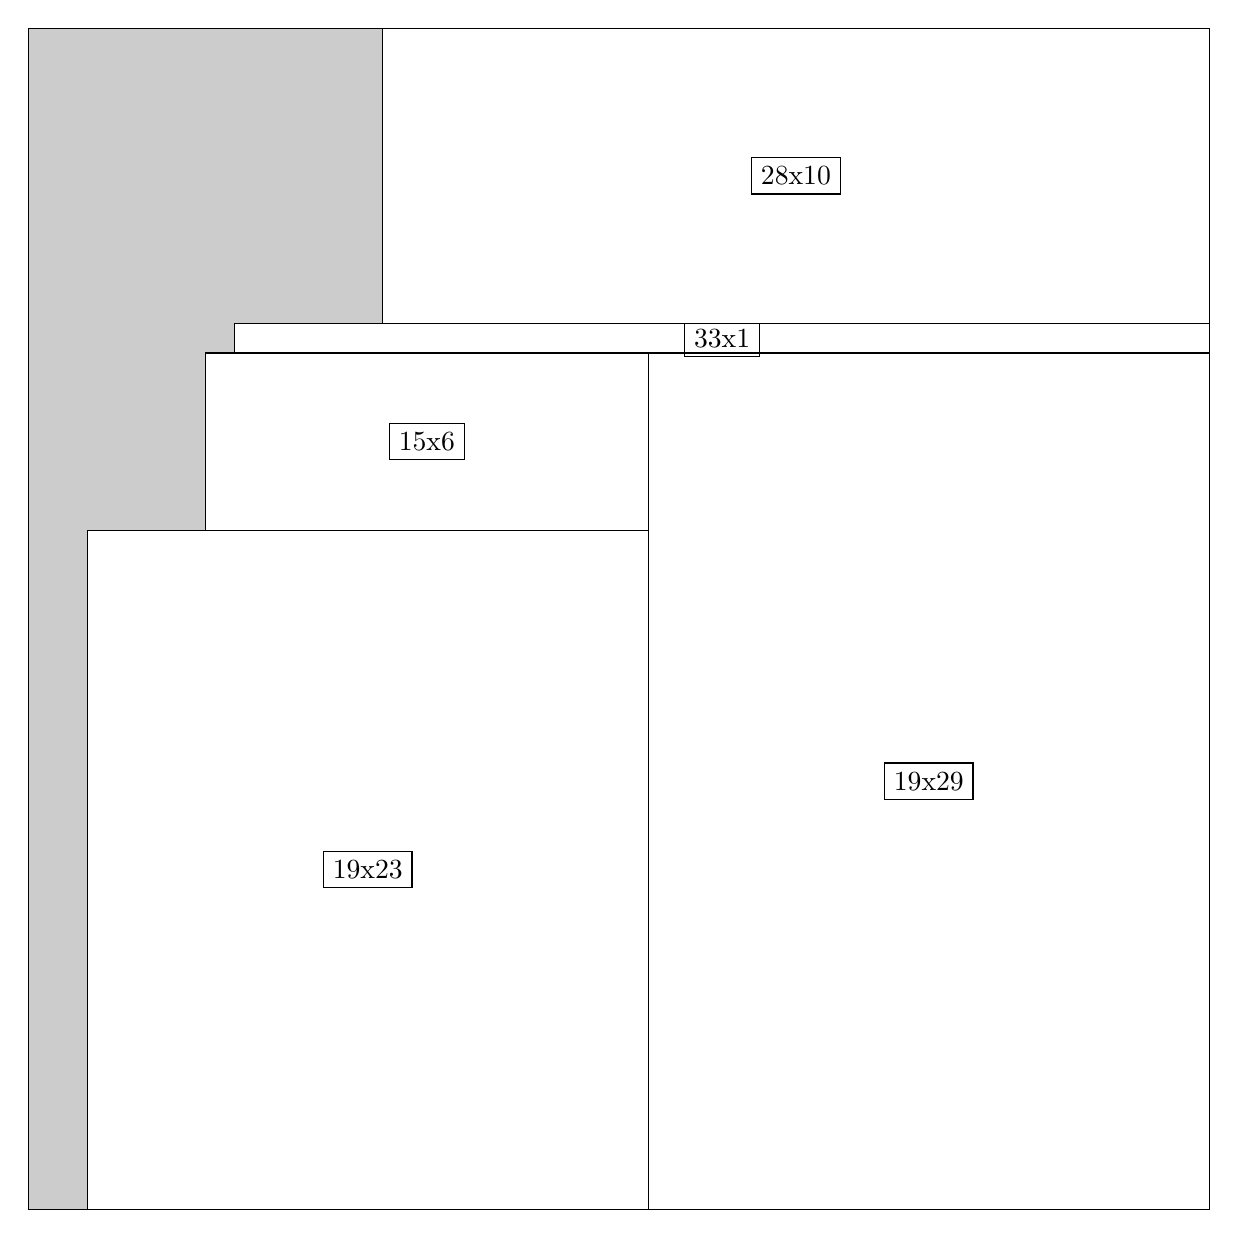
\begin{tikzpicture}[shorten >=1pt,scale=1.0,every node/.style={scale=1.0},->]
\tikzstyle{vertex}=[circle,fill=black!25,minimum size=14pt,inner sep=0pt]
\filldraw[fill=gray!40!white, draw=black] (0,0) rectangle (15.0,15.0);
\foreach \name/\x/\y/\w/\h in {19x29/7.875/0.0/7.125/10.875,19x23/0.75/0.0/7.125/8.625,15x6/2.25/8.625/5.625/2.25,33x1/2.625/10.875/12.375/0.375,28x10/4.5/11.25/10.5/3.75}
\filldraw[fill=white!40!white, draw=black] (\x,\y) rectangle node[draw] (\name) {\name} ++(\w,\h);
\end{tikzpicture}


w =19 , h =29 , x =21 , y =0 , v =551
\par
w =19 , h =23 , x =2 , y =0 , v =437
\par
w =15 , h =6 , x =6 , y =23 , v =90
\par
w =33 , h =1 , x =7 , y =29 , v =33
\par
w =28 , h =10 , x =12 , y =30 , v =280
\par
\newpage


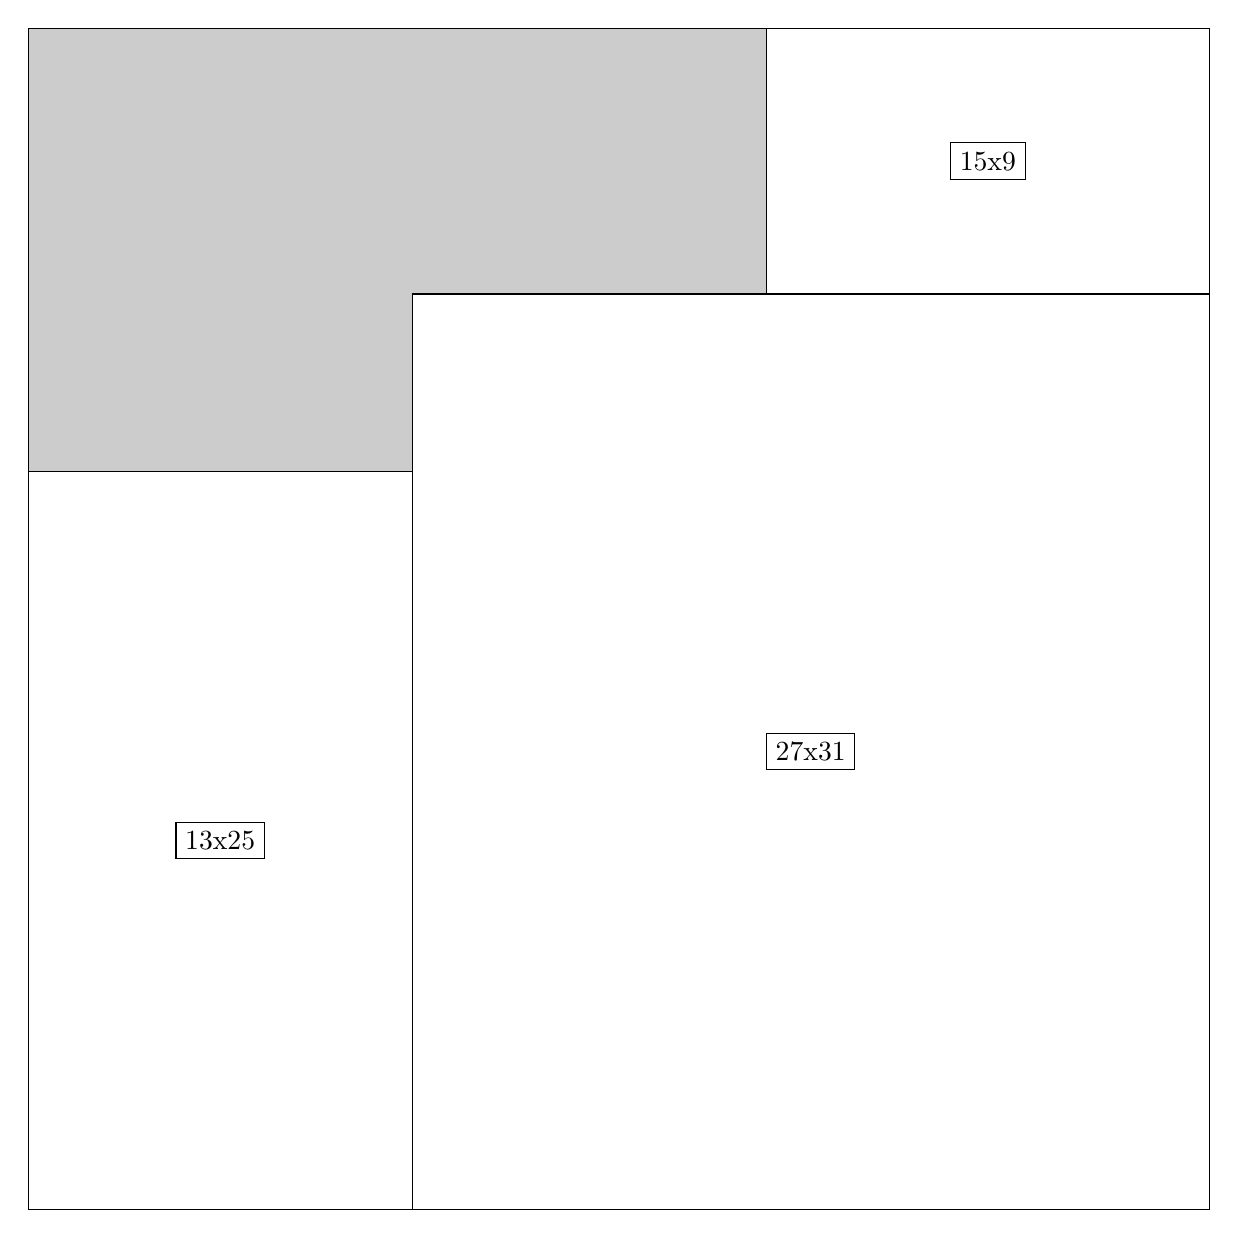
\begin{tikzpicture}[shorten >=1pt,scale=1.0,every node/.style={scale=1.0},->]
\tikzstyle{vertex}=[circle,fill=black!25,minimum size=14pt,inner sep=0pt]
\filldraw[fill=gray!40!white, draw=black] (0,0) rectangle (15.0,15.0);
\foreach \name/\x/\y/\w/\h in {27x31/4.875/0.0/10.125/11.625,13x25/0.0/0.0/4.875/9.375,15x9/9.375/11.625/5.625/3.375}
\filldraw[fill=white!40!white, draw=black] (\x,\y) rectangle node[draw] (\name) {\name} ++(\w,\h);
\end{tikzpicture}


w =27 , h =31 , x =13 , y =0 , v =837
\par
w =13 , h =25 , x =0 , y =0 , v =325
\par
w =15 , h =9 , x =25 , y =31 , v =135
\par
\newpage


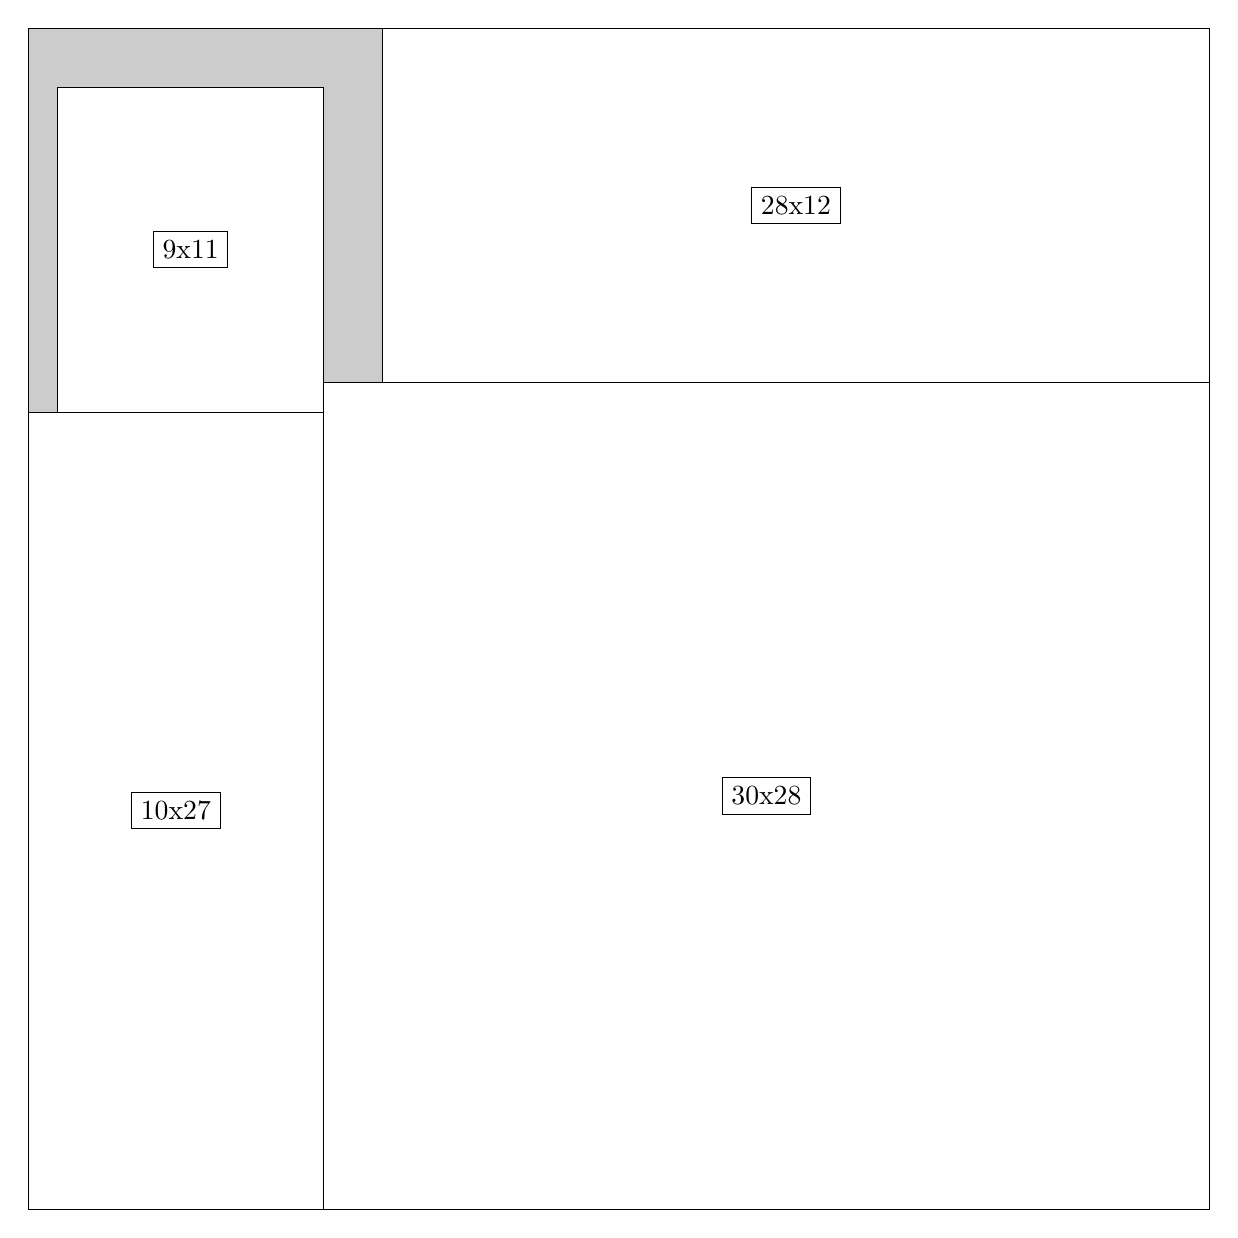
\begin{tikzpicture}[shorten >=1pt,scale=1.0,every node/.style={scale=1.0},->]
\tikzstyle{vertex}=[circle,fill=black!25,minimum size=14pt,inner sep=0pt]
\filldraw[fill=gray!40!white, draw=black] (0,0) rectangle (15.0,15.0);
\foreach \name/\x/\y/\w/\h in {30x28/3.75/0.0/11.25/10.5,28x12/4.5/10.5/10.5/4.5,10x27/0.0/0.0/3.75/10.125,9x11/0.375/10.125/3.375/4.125}
\filldraw[fill=white!40!white, draw=black] (\x,\y) rectangle node[draw] (\name) {\name} ++(\w,\h);
\end{tikzpicture}


w =30 , h =28 , x =10 , y =0 , v =840
\par
w =28 , h =12 , x =12 , y =28 , v =336
\par
w =10 , h =27 , x =0 , y =0 , v =270
\par
w =9 , h =11 , x =1 , y =27 , v =99
\par
\newpage


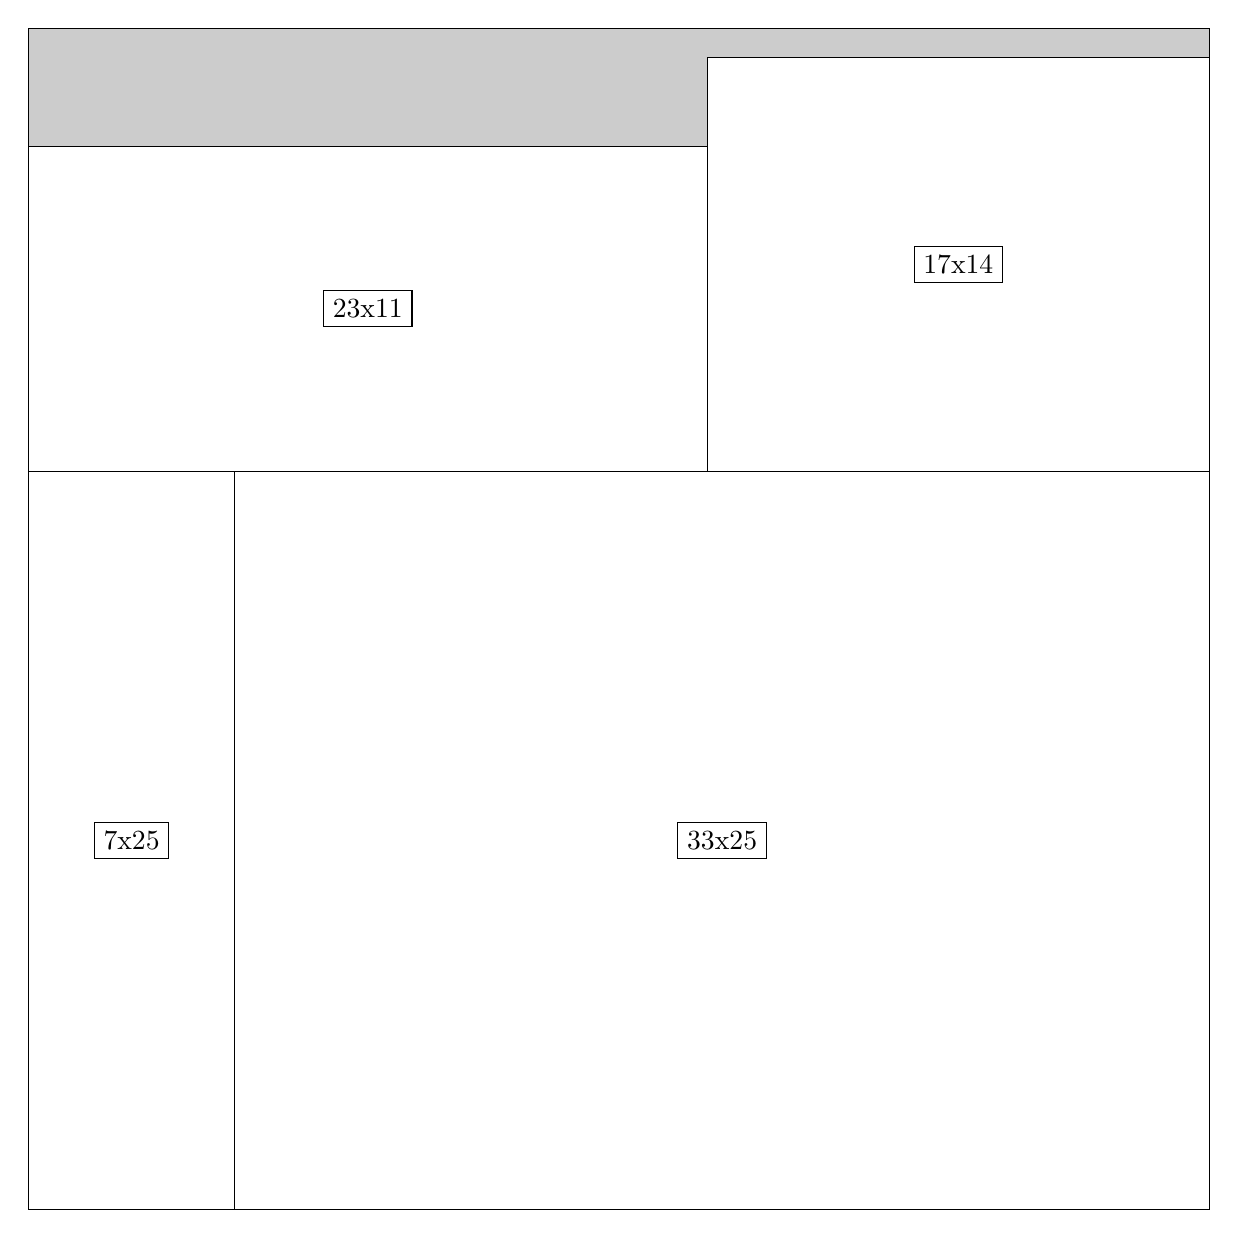
\begin{tikzpicture}[shorten >=1pt,scale=1.0,every node/.style={scale=1.0},->]
\tikzstyle{vertex}=[circle,fill=black!25,minimum size=14pt,inner sep=0pt]
\filldraw[fill=gray!40!white, draw=black] (0,0) rectangle (15.0,15.0);
\foreach \name/\x/\y/\w/\h in {33x25/2.625/0.0/12.375/9.375,7x25/0.0/0.0/2.625/9.375,17x14/8.625/9.375/6.375/5.25,23x11/0.0/9.375/8.625/4.125}
\filldraw[fill=white!40!white, draw=black] (\x,\y) rectangle node[draw] (\name) {\name} ++(\w,\h);
\end{tikzpicture}


w =33 , h =25 , x =7 , y =0 , v =825
\par
w =7 , h =25 , x =0 , y =0 , v =175
\par
w =17 , h =14 , x =23 , y =25 , v =238
\par
w =23 , h =11 , x =0 , y =25 , v =253
\par
\newpage


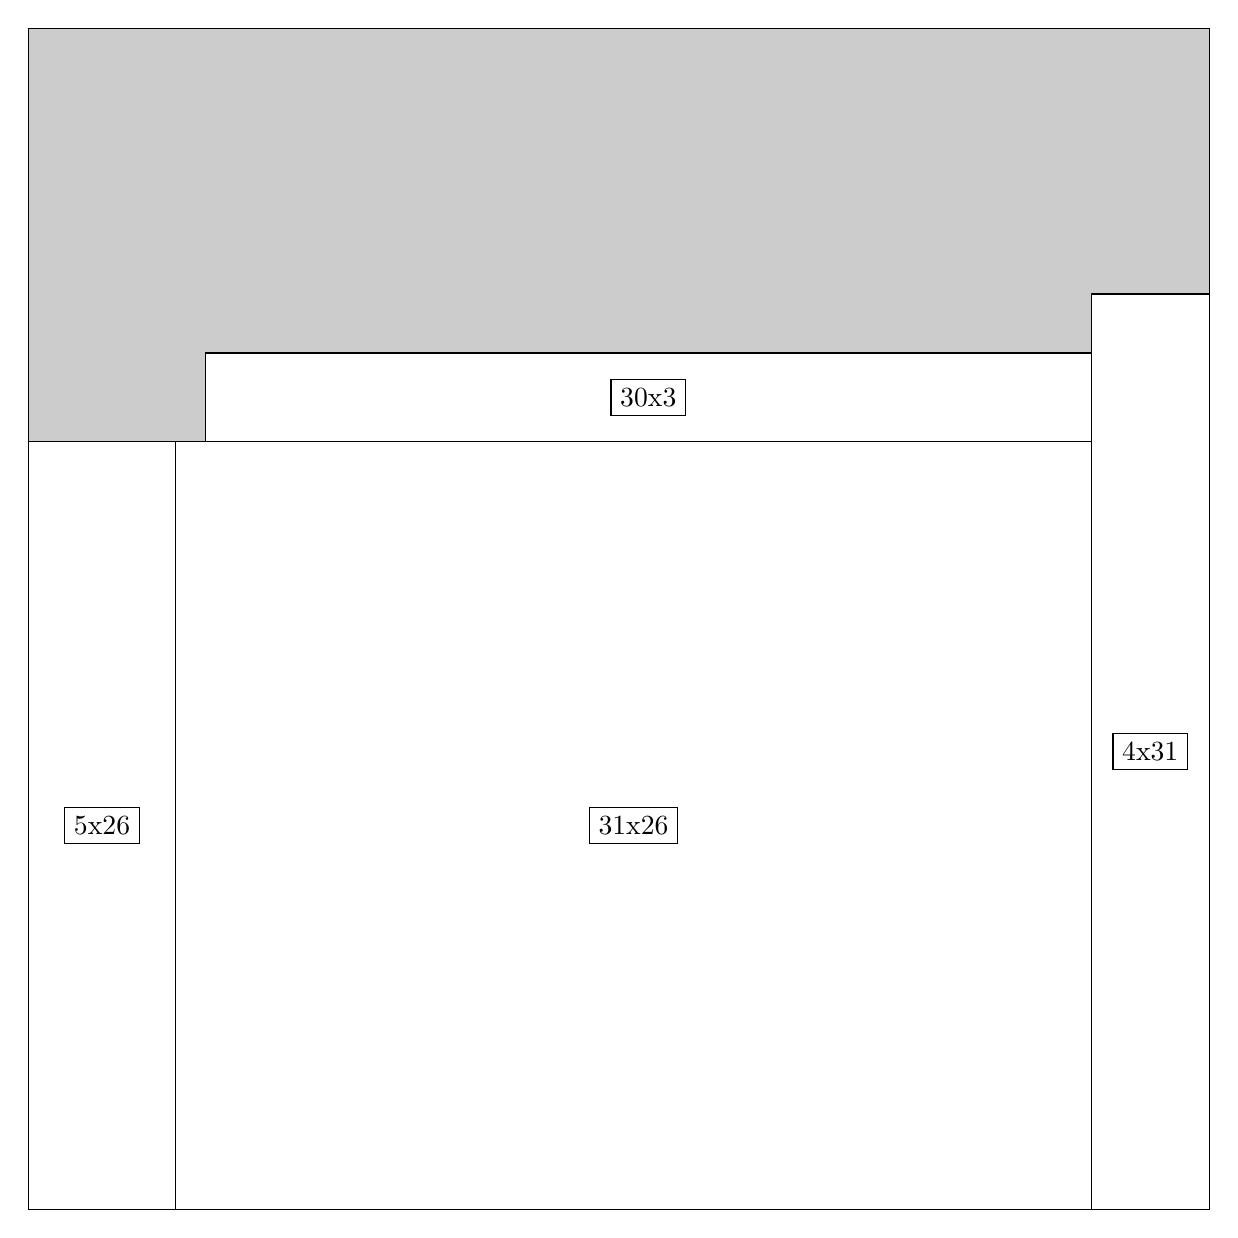
\begin{tikzpicture}[shorten >=1pt,scale=1.0,every node/.style={scale=1.0},->]
\tikzstyle{vertex}=[circle,fill=black!25,minimum size=14pt,inner sep=0pt]
\filldraw[fill=gray!40!white, draw=black] (0,0) rectangle (15.0,15.0);
\foreach \name/\x/\y/\w/\h in {4x31/13.5/0.0/1.5/11.625,31x26/1.875/0.0/11.625/9.75,30x3/2.25/9.75/11.25/1.125,5x26/0.0/0.0/1.875/9.75}
\filldraw[fill=white!40!white, draw=black] (\x,\y) rectangle node[draw] (\name) {\name} ++(\w,\h);
\end{tikzpicture}


w =4 , h =31 , x =36 , y =0 , v =124
\par
w =31 , h =26 , x =5 , y =0 , v =806
\par
w =30 , h =3 , x =6 , y =26 , v =90
\par
w =5 , h =26 , x =0 , y =0 , v =130
\par
\newpage


\end{document}